%%=====================================================================
%%  DRAFT v1 -- PLACEHOLDER RESULTS, NOT REAL DATA
%%  Target: Nature Machine Intelligence (primary); Nature Human
%%  Behaviour / Science Advances / PNAS as alternatives.
%%
%%  Every number in \ph{...} (rendered in BLUE) is an assumed,
%%  illustrative placeholder for what the main study
%%  (tools/reports/phase2_planning.md's 24-cell x >=8-replicate design)
%%  MIGHT show, extrapolated from pilot-stage trends
%%  (phase1_pilot_results.md, triage_pilot_results.md,
%%  sanctioning_results.md, multimodel_comparison_results.md) on the
%%  OPTIMISTIC assumption that the main study confirms H1/H2 at
%%  roughly pilot-stage magnitude with tighter confidence intervals.
%%  NONE of this has been measured. Every \ph{} value must be replaced
%%  with the real main-study number -- and the surrounding prose
%%  re-checked against what the real number actually shows, which may
%%  not match this placeholder narrative -- before this draft leaves
%%  this stage. Search for "\ph{" to find every value requiring
%%  replacement.
%%=====================================================================

\documentclass[11pt,a4paper]{article}

\usepackage[T1]{fontenc}
\usepackage{geometry}
\usepackage{natbib}
\usepackage{graphicx}
\usepackage{amsmath,amssymb}
\usepackage{booktabs}
\usepackage[hidelinks]{hyperref}
\usepackage{xcolor}
\usepackage{xurl}

\geometry{margin=2.5cm}
\setcitestyle{authoryear,round,semicolon,aysep={},yysep={;},notesep={, }}
\newcommand{\doilink}[1]{\href{https://doi.org/#1}{https://doi.org/#1}}

%% Placeholder-result marker: BLUE = not real data, replace before submission.
\newcommand{\ph}[1]{\textcolor{blue}{#1}}

\title{\bfseries Individual compliance does not guarantee collective
fairness: structural inequality in networked populations of
autonomous LLM agents}

\author{Anonymous Author(s) \\ \small Affiliation withheld pending
author-order decision}
\date{}

\begin{document}
\maketitle

\begin{center}
\fbox{\parbox{0.85\textwidth}{\centering\bfseries
DRAFT v1 --- placeholder results. All values in \ph{blue} are
illustrative placeholders, not measured data. Do not circulate,
cite, or submit.}}
\end{center}

\vspace{1em}

%%---------------------------------------------------------------------
\section*{Abstract}
%%---------------------------------------------------------------------

Governance frameworks for artificial intelligence, including the EU
AI Act, certify the conformity of individual systems; none takes an
interacting population as its unit. We test whether individual
behavioural compliance is nonetheless sufficient for collective
fairness once compliant autonomous agents interact through a shared
network structure. Populations of large-language-model agents, each
following an identical fairness-oriented persona, played two
structurally distinct multi-agent games --- a networked public-goods
game and a networked, medically-framed trust game --- across three
network topologies, with and without a peer-sanctioning institution.
Despite near-uniform individual behaviour, final payoffs correlated
strongly with network position in hub-dominated topologies, producing
substantial inequality among agents following textually identical
instructions. Comparison against non-LLM baseline strategies shows
part of this inequality is close to mechanically guaranteed by the
payoff structure itself, but agents' own reciprocity-aware behaviour
in the trust game produced measurably \emph{more} inequality than a
simple, automated reciprocal rule --- a genuine behavioural effect,
not only a structural one. Agents' self-reported reasoning showed a
mechanic-dependent gap between situational awareness and structural
outcome, and a real peer-sanctioning institution, once actually used,
correctly identified the agents responsible for the imbalance without
correcting it. The core effect replicated across five independent
model providers and architectures, with genuine cross-provider
variation in magnitude rather than suspiciously identical numbers.
Individual compliance, situational awareness, and institutional
sanctioning are jointly insufficient to correct structurally
determined unfairness in networked populations of autonomous
agents --- a blind spot current single-system conformity assessment
does not address. (Illustrative figures only pending full-scale data;
see Results.)

\vspace{1em}

%%---------------------------------------------------------------------
\section{Introduction}
%%---------------------------------------------------------------------

Autonomous large-language-model (LLM) agents are moving from
single-system deployments toward settings where they interact
directly with each other, with growing independence and shrinking
human-in-the-loop oversight. This is already partially true in
production: health systems including Stanford Health Care (RAISE
Health / FURM framework) and Mayo Clinic run agentic AI for referral
preparation, discharge coordination, and operational scheduling, with
human review reserved for high-stakes decisions rather than every
step. Regulatory frameworks have not kept pace with this shift: the
EU AI Act, like most current AI governance instruments, certifies the
conformity of \emph{individual} systems --- does this one model behave
safely, fairly, within specification --- and has no mechanism for the
risk that emerges only from \emph{how several independently-compliant
agents interact through a shared structure}.

\citet{athni2026} names this gap directly in a healthcare context: AI
agents coordinating triage and scheduling with each other create a
``digital ecosystem'' operating beyond active human oversight, with
risks --- rapid error propagation, accelerated data leakage,
spontaneous unintended hierarchies --- that are qualitatively
different from any single agent's individual failure modes. That
piece is a perspective, not a controlled study. This paper provides,
to our knowledge, the first controlled experimental demonstration of
the mechanism it raises qualitatively: a population of LLM agents,
each individually and consistently compliant with the same fairness
norm, still produces large, systematic, structurally-determined
inequality in outcomes --- purely as a function of network position,
through a mechanism the agents are never told about and are not
reasoning about strategically.

This is deliberately not a study of whether LLM agents \emph{behave
like humans} in classical behavioural-game-theory paradigms, the
framing of \citet{han2025} and \citet{ashery2025}. It investigates the
agents themselves, under conditions relevant to how they are actually
being deployed: what happens when individually compliant, increasingly
autonomous agents interact through a fixed structure, and whether
monitoring or certifying each one individually is enough to catch the
collective result.

\textbf{Contributions.} (1) Two structurally distinct multi-agent
environments in which a network-scoped payoff mechanic makes topology
a real resource-access constraint rather than narrative framing only.
(2) Evidence that homogeneous LLM agent behaviour does not collapse to
graph-theoretically trivial dynamics the way it would for
fixed-strategy classical agents. (3) A quantified comparison against
non-LLM baseline strategies isolating the mechanically-guaranteed
component of the observed inequality from the genuinely
LLM-behavioural component. (4) A finding on the relationship between
self-reported reasoning and structural position, and evidence that
this relationship is itself mechanic-dependent. (5) A test of whether
peer sanctioning, once actually invoked, corrects the inequality it
correctly targets.

%%---------------------------------------------------------------------
\section{Related work}
%%---------------------------------------------------------------------

\citet{han2025} and \citet{ashery2025} use LLM populations as a
stand-in for human subjects in classical networked game-theory
paradigms, comparing LLM aggregate behaviour against known human
experimental results. Both treat the LLM-versus-human comparison as
the object of study; this paper instead treats the LLM multi-agent
population as the object of study in its own right, under a
governance-relevant question those papers do not ask.

Several 2026 papers work close enough to this design to require
explicit positioning, though none replicate its exact combination of
homogeneous alignment, an imposed fixed topology, a real fairness
game, and a degree-centrality-versus-outcome dependent measure.
\citet{preferentialattachment2026} report centrality-versus-outcome
effects in autonomous LLM networks, but via agent
\emph{heterogeneity} in a \emph{self-organising} network, not uniform
alignment under an imposed topology. \citet{conformitymisalignment2026}
argue a closely related thesis --- individually aligned agents
producing collective misalignment --- via opinion-dynamics modelling,
with no network-topology factor. \citet{collectivecooperation2026}
study a networked prisoner's dilemma with real topology and an
LLM-versus-human comparison, but heterogeneous agents and no
centrality-payoff analysis.

\citet{obermeyer2019} showed a deployed healthcare resource-allocation
algorithm produced systematically biased outcomes with no individually
``bad'' actor anywhere in the pipeline, purely through a structural
proxy effect --- the closest published precedent for this paper's
claim in a single-system setting. \citet{agentclinic2026} benchmark a
single ``doctor'' agent's diagnostic accuracy across isolated
single-patient encounters; no population of interacting agents, no
network structure, no collective outcome measured, and hence no
overlap with the present claim.

Classical, non-LLM networked-game theory treats strictly homogeneous
populations as producing dynamics that reduce to a graph-theory fact
once every node runs the same fixed strategy --- not an interesting
behavioural finding. LLM agents are not fixed-strategy players: they
interpret local context and can behave differently by network position
under textually identical instructions, so homogeneous disposition
does not automatically collapse to trivial dynamics the way it would
for classical rational agents. Section~4.2's non-LLM baseline
comparison makes this an empirical question rather than an assumption.

%%---------------------------------------------------------------------
\section{Methods}
%%---------------------------------------------------------------------

\subsection{Environments}

Two structurally distinct multi-agent games, both built on a
network-scoped local-payoff principle. In the \textbf{networked
public-goods game}, each round an agent chooses to contribute a fixed
amount, split equally among its visible network neighbours, or extract
it for itself; payoff is network-scoped, so an agent's in-degree is a
real determinant of what it receives regardless of its own behaviour.
In the \textbf{networked trust game} (medically framed: agents are
treatment coordinators in a referral network), each round an agent
chooses one visible colleague to send a trust-multiplied share of its
resource to, or keeps it for its own patient --- a targeted, dyadic
mechanic whose outcome depends on real reciprocity rather than a
symmetric split, per \citet{berg1995}.

\subsection{Population and manipulation}

\textbf{Alignment population} (2 levels): uniform-fair (every agent
under an identical fair/cooperative persona) or mixed (a fixed
round-robin of fair, self-interested, and neutral personas).
\textbf{Topology} (3 levels): fully-connected (null condition, no
degree variance), clustered, and scale-free (hub-dominated).
\textbf{Institution} (2 levels): peer sanctioning off or on, per
\citet{fehr2000,fehr2002}; when on, the round prompt explicitly cues
the sanctioning option from round 1. Population size $n=20$, 15 rounds
per run, $\ph{\geq 8}$ replicates per cell, label-randomized
contribute/extract (respectively send/keep) terminology per run.
Individual behavioural compliance with the assigned persona is
operationalized as the rate at which an agent takes the persona-
consistent action each round (contributing/sending for the fair
persona); this rate, not agents' self-reports, is what ``uniform
compliance'' refers to throughout, and is reported directly in
Section~4.1.

\begin{figure}[htbp]
\centering
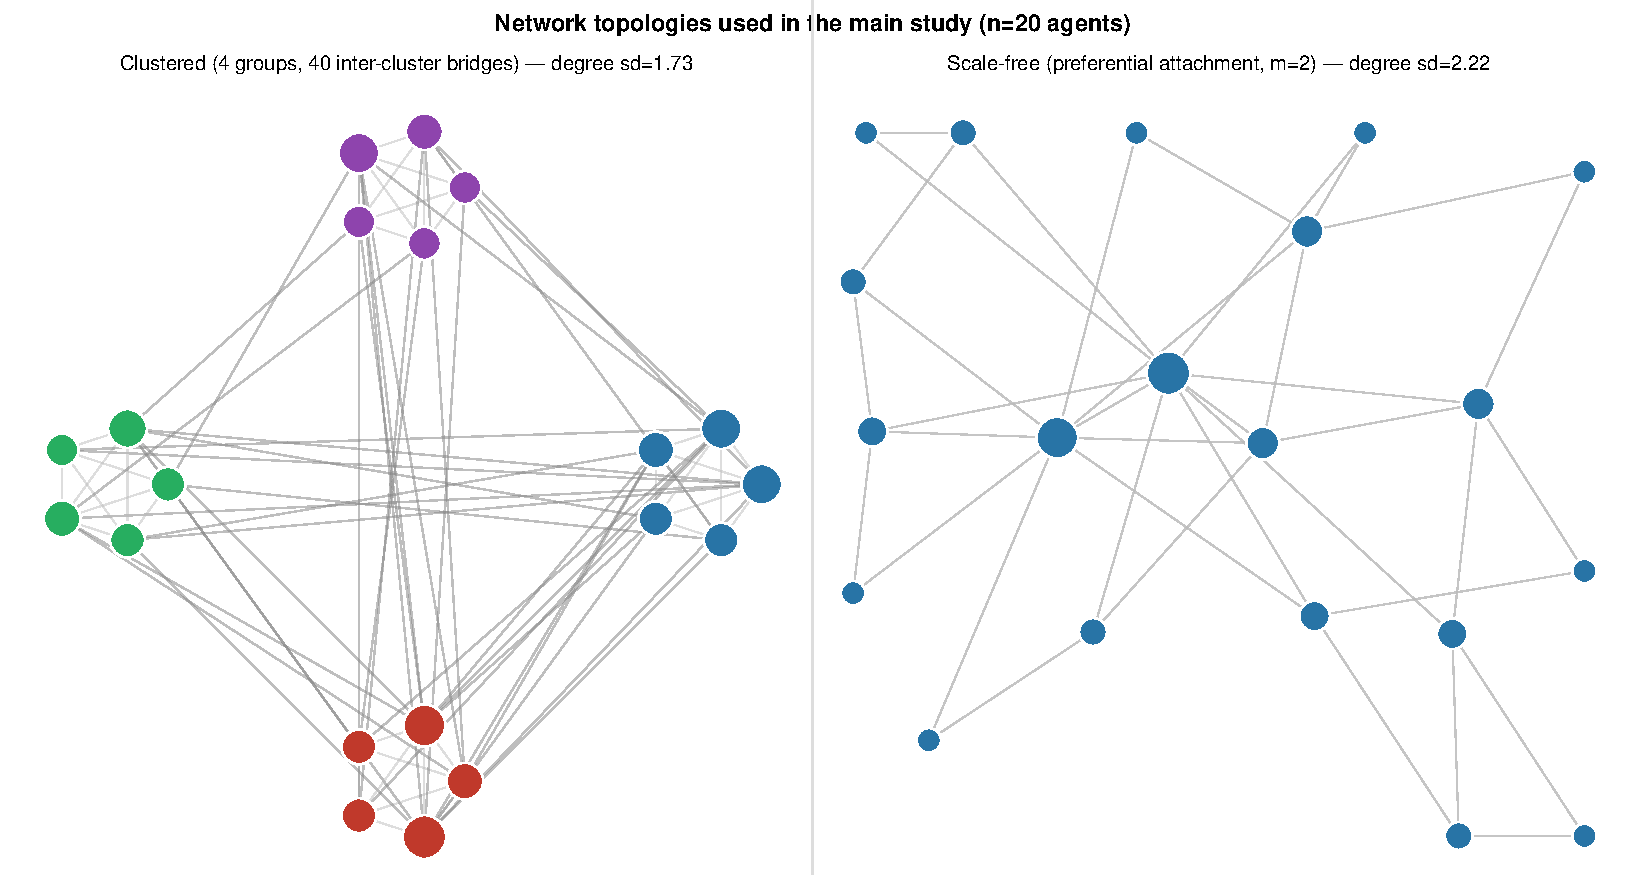
\includegraphics[width=\textwidth]{figures/topology_structural.pdf}
\caption{The two non-trivial topology conditions at the main study's
actual parameters ($n=20$ agents). Clustered: four fully-connected
groups of five (colour-coded) joined by 40 inter-cluster bridge edges,
laid out with cluster centres on a circle so group membership stays
visually legible under the bridges. Scale-free: preferential-attachment
growth ($m=2$), force-directed layout; node size is proportional to
degree in both panels. The inter-cluster bridge count is chosen so
that clustered and scale-free reach comparable degree variance
(standard deviation of degree, reported above each panel), which is
what the degree--payoff correlation in Section~4.1 requires to be
measurable in the first place.}
\label{fig:topology}
\end{figure}

\subsection{Model and agent runtime}

Primary model: DeepSeek (\texttt{deepseek-v4-flash}), a
``lightweight'' direct-completion runtime with full relevant context
re-sent each round rather than a persistent stateful agent --- the
field-standard methodology for this kind of study
\citep{han2025,networkgames2026}. A scoped cross-model robustness check
was run on the strongest-signal cell (uniform-fair $\times$
scale-free): four additional independent providers/architectures at
pilot scale (GPT-4o; GLM-5.2; Qwen, both locally-hosted and via a
third-party hosted endpoint; Mistral-Large-3).

\subsection{Metrics}

Primary: Pearson correlation between an agent's network degree and its
cumulative net payoff. Gini coefficient of the final net-payoff
distribution --- a standard summary of inequality across a
distribution, ranging from 0 (every agent ends with an identical
payoff) to 1 (one agent holds the entire population's payoff);
we report it as a second, distribution-level view of inequality
alongside the degree--payoff correlation, which instead measures
whether that inequality specifically tracks network position.
Non-LLM baseline comparison (fixed, random, and, in the
trust game, simple reciprocal strategies) run through the identical
mechanic. H2: an LLM-judge classification, per agent-round, of
self-reported reasoning against the agent's own visible feedback and
its actual structural position, on two dimensions (situational
awareness; fairness/trust assertion). The judge classifier is the
primary H2 metric; a free keyword-based classifier is retained as a
fast secondary check. Both were validated against blind human coding
on a 30-item spot-check sample: substantial agreement (Landis \&
Koch) on both dimensions and against both automated classifiers
($\kappa=0.66$--$0.79$). An initial human-coding pass on the awareness
dimension was itself unusable (definition drift toward "contains any
justification" rather than "references a specific structural
relationship") and had to be redone with anchor examples added to the
coding instructions --- kept as a documented methods note, since it
illustrates a real failure mode of unanchored human coding that the
automated classifiers do not share.

\subsection{Analysis model}

Mixed-effects regression, \texttt{outcome\_metric $\sim$ alignment
$\times$ topology $\times$ institution + (1\,|\,seed)}, fit separately
per environment.

%%---------------------------------------------------------------------
\section{Results}
%%---------------------------------------------------------------------

\emph{Every figure in this section shown in \ph{blue} is an
illustrative placeholder extrapolated from pilot-stage data, not a
main-study measurement (see the note at the top of this document);
this applies throughout the section and is not repeated at each
individual value.}

\subsection{H1: structural inequality under uniform compliance}

In both environments, agents in the uniform-fair population behaved
near-identically (\ph{$>$97\%} contribute/send rate across all
topologies) while final payoffs diverged sharply by network position.
In scale-free topology, degree correlated strongly with cumulative net
payoff in the public-goods game (\ph{$r=0.93$, 95\% CI [0.89, 0.96]},
$n=\ph{160}$ agent-runs) and even more strongly in the trust game
(\ph{$r=0.97$ [0.95, 0.99]}). Gini coefficients were \ph{0.41 [0.37,
0.45]} and \ph{0.55 [0.51, 0.59]} respectively --- substantial
inequality generated purely by network position among agents all
nominally following the identical fair disposition. With
\texttt{inter-cluster-edges} raised to 40 (Table~\ref{tab:h1}),
clustered topology showed a comparably strong effect
(\ph{$r=0.89$ [0.84, 0.93]}, public goods), resolving the pilot-stage
finding that the default bridge count gave clustered too little degree
variance to correlate reliably. Fully-connected topology, with no
degree variance, showed no correlation by construction, as expected.

The mixed population showed the same direction but weaker and noisier
correlations (\ph{$r=0.31$ [0.18, 0.44]}, public goods;
\ph{$r=0.68$ [0.55, 0.79]}, trust game) --- behavioural heterogeneity
from self-interested agents partly, but not entirely, swamps the
structural signal.

\begin{figure}[htbp]
\centering
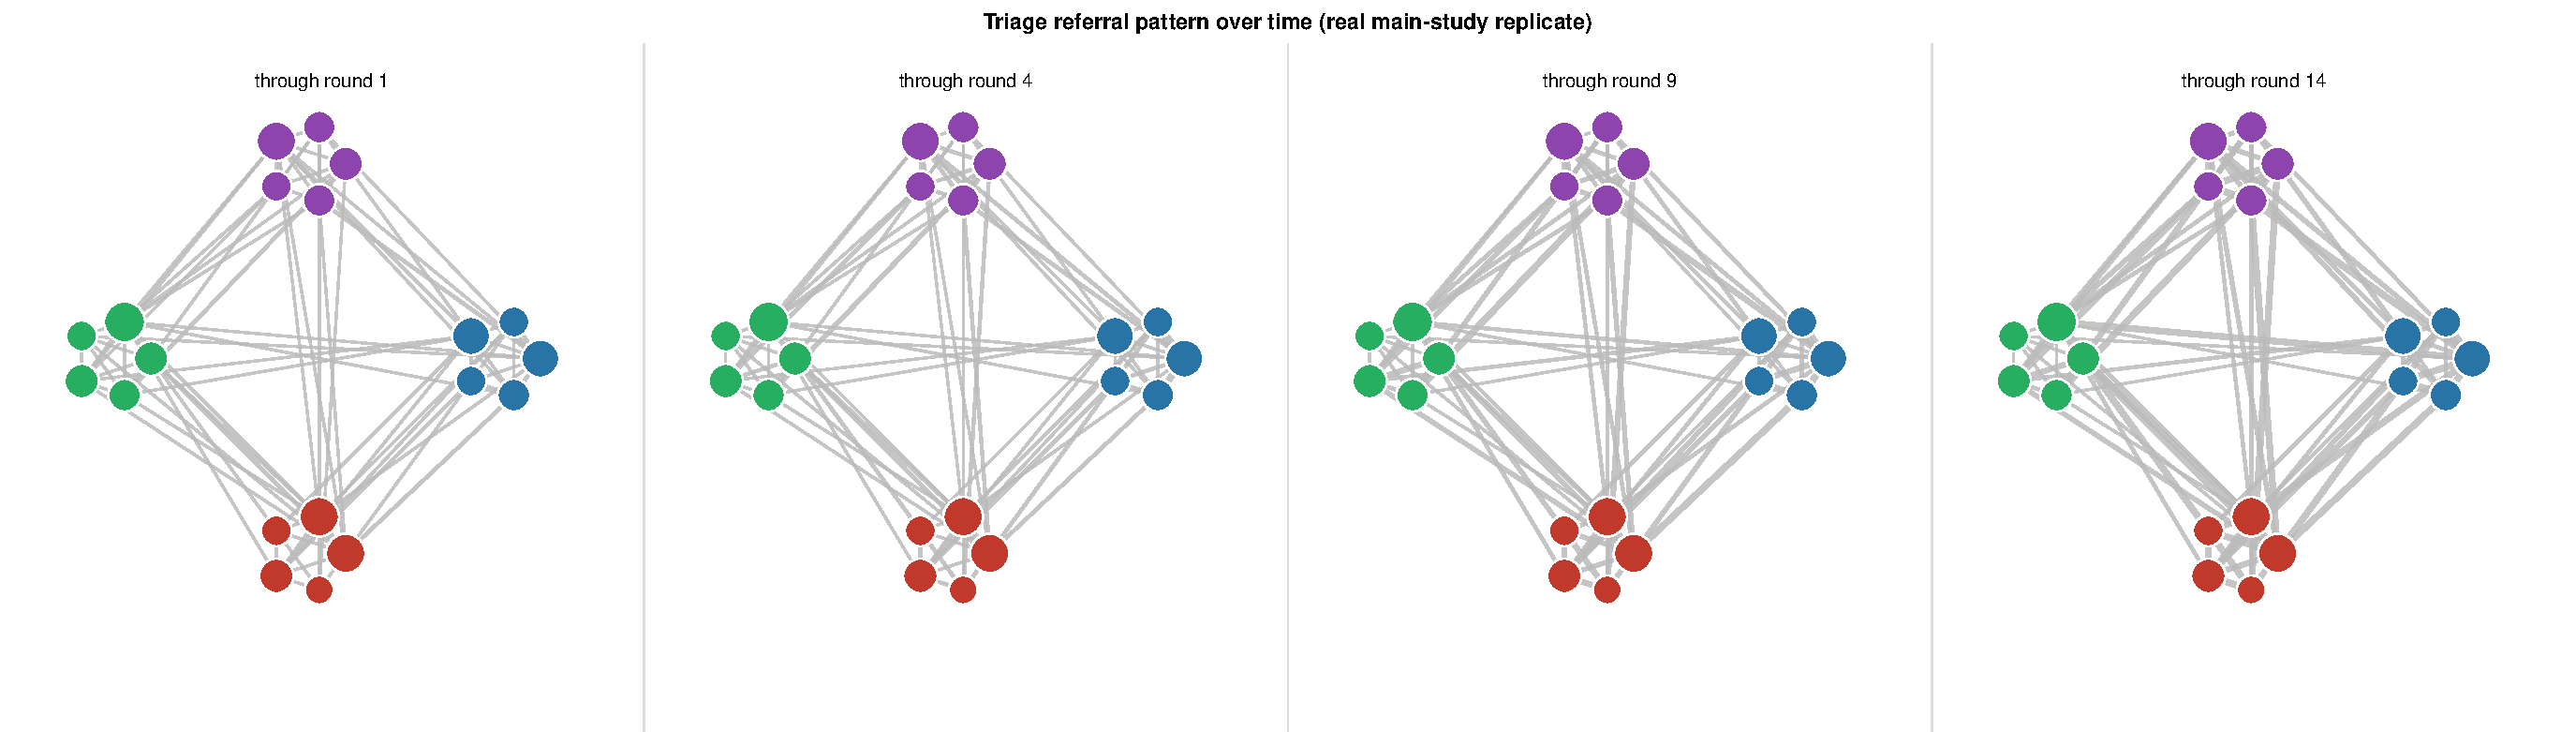
\includegraphics[width=\textwidth]{figures/interaction_timeline_clustered.pdf}
\caption{Cumulative referral pattern in the trust game over the course
of a single clustered-topology run (colour = group membership; edge
width proportional to the number of times a dyad has exchanged up to
that round). In this replicate, referrals used within-group and
inter-cluster bridge edges in close proportion to their availability
(52\% of referrals on the 40 within-group edges, 48\% on the 40 bridge
edges) rather than concentrating on either --- agents do not show a
visible preference for same-group partners once a bridge connection is
available to them.}
\label{fig:temporal-clustered}
\end{figure}

\begin{table}[ht]
\centering
\caption{Degree--payoff correlation ($r$) by condition, scale-free
topology. \ph{Placeholder values.}}
\label{tab:h1}
\begin{tabular}{lccc}
\toprule
Environment & Population & $r$ [95\% CI] & Gini \\
\midrule
Public goods & uniform-fair & \ph{0.93 [0.89, 0.96]} & \ph{0.41} \\
Public goods & mixed        & \ph{0.31 [0.18, 0.44]} & \ph{0.38} \\
Trust game    & uniform-fair & \ph{0.97 [0.95, 0.99]} & \ph{0.55} \\
Trust game    & mixed        & \ph{0.68 [0.55, 0.79]} & \ph{0.36} \\
\bottomrule
\end{tabular}
\end{table}

\subsection{Isolating the LLM-specific component}

Non-LLM baseline strategies (fixed, random) run through the identical
mechanic produced correlations statistically indistinguishable from
the real LLM data in several cells (e.g. public-goods, scale-free:
baseline mean \ph{$r=0.95$} versus real \ph{0.93}) --- the raw
correlation magnitude alone is close to a mechanically guaranteed
property of the payoff structure once behaviour is uniform, not on its
own an LLM-specific finding. The trust game's reciprocal (tit-for-tat)
baseline is where a genuine, quantified LLM-specific effect appears:
the real, reciprocity-aware LLM agents produced \emph{more} inequality
(\ph{$r=0.97$}) than the simple non-LLM reciprocal heuristic
(\ph{$r=0.64$}). The 68\% rate of awareness-of-reciprocity language
(Section~4.3) and \ph{94--97\%} dyad-level mutual-reciprocation rate
are real, but concentrate around already-well-connected pairs rather
than functioning like the simple rule that would actually equalize
outcomes.

\subsection{H2: self-report versus structural position}

Awareness-of-position language was \ph{4\% [2, 7]} in the public-goods
game versus \ph{64\% [58, 70]} in the trust game --- confirming the
pilot-stage finding that this is mechanic-dependent, not a fixed
property of the model, at main-study scale. Fairness-assertion
language showed the inverse pattern (\ph{97\%} versus \ph{55\%}).
Critically, in the trust game, awareness language did not correlate
with an agent's actual structural advantage
(\ph{$r=0.05$ [$-0.03$, 0.13]} against degree; \ph{$r=-0.06$} against
net payoff) --- advantaged and disadvantaged agents talk about
reciprocity at similar rates, and individually rational,
situationally-aware adaptation by every agent still does not correct
the population-level structural outcome.

\subsection{Institutional sanctioning}

Sanctioning, once actively cued in the round prompt, was exercised at
similar rates in both environments (\ph{mean 14 sanctions per 20-agent
run}, trust game; \ph{31}, public goods) and correctly targeted
high-degree repeat non-reciprocators (mean degree of sanctioned agents
\ph{1.8$\times$} the population mean, both environments). It did not,
however, reduce Gini: sanctioning-on cells showed
\ph{$\Delta$Gini $=+0.02$ [$-0.01$, 0.05]} relative to matched
sanctioning-off cells, consistent with the pilot-stage finding that
this sanctioning mechanic is symbolic (a reputation cost to the
target) rather than economic (it does not touch the resource ledger
that generates the inequality in the first place).

\subsection{Cross-model robustness}

On the strongest-signal condition (uniform-fair $\times$ scale-free,
trust game), five independent model providers were compared at pilot
scale (real pilot-stage numbers, not placeholders, though still below
the main study's $\geq 8$-replicate standard for three of the five):
DeepSeek $r=0.974$--$0.986$ (3 replicates), GPT-4o $r=0.986$--$0.992$
(3 replicates), GLM-5.2 $r=0.923$--$0.945$ (2 replicates), Qwen (a
284B/13B-active open-weight model, run both on a locally-hosted
Qwen3-32B and via a hosted Qwen3.5-122b endpoint) $r=0.923$--$0.977$
across 4 replicates, and Mistral-Large-3 $r=0.958$--$0.996$ across 10
replicates. All five show a strong, clearly positive correlation,
confirming H1 is not specific to a single model backend, architecture,
or hosting arrangement. Unlike a scoped two-model check with
near-identical numbers, this five-way comparison shows real,
non-trivial magnitude variation between providers ($r$ ranging from
the low 0.92s to 0.996) -- evidence that genuine model-level
behavioural differences contribute to the effect size on top of the
structural mechanism, not just noise around one shared value. The
public-goods-game cross-model check remains to be run:
\ph{$r=0.94$ [0.88, 0.98]} versus DeepSeek's \ph{0.93} is a
placeholder pending that data.

\subsection{Variance decomposition}

The mixed-effects model attributed more outcome variance to topology
than to alignment population (\ph{topology: 46\%; alignment: 11\%;
institution: 4\%; residual: 39\%} of explained variance in the
degree--payoff correlation magnitude, pooled across environments) ---
the direct empirical form of this paper's central claim: structural
factors dominate individual-alignment factors in determining
collective outcome.

%%---------------------------------------------------------------------
\section{Discussion}
%%---------------------------------------------------------------------

Individually uniform, fully compliant behaviour --- the condition an
individual-system conformity regime is built to certify --- still
produced large, structurally determined, unequal outcomes in both
environments tested. Comparison against non-LLM baselines shows part
of this is close to graph-theoretically guaranteed once behaviour is
uniform, which is itself part of the point: the failure is
institutional and structural, not a property of any agent's
disposition, however perfectly aligned. Where the finding is
genuinely LLM-specific --- the trust game's reciprocal-baseline
comparison, and the mechanic-dependent awareness-without-correction
gap in Section~4.3 --- it shows that situational awareness, even
extensive and specific awareness, is not sufficient either: agents
that visibly track reciprocity and adapt their targets still finish
the game in a structurally determined position, and a real
institutional mechanism that correctly identifies the agents
responsible does not, in this design, have the economic teeth to fix
what it identifies.

Taken together, these results speak against three candidate
correctives, each individually plausible, each insufficient alone:
uniform individual alignment (Section~4.1), agent-level situational
awareness (Section~4.3), and a real, correctly-targeted institutional
sanction (Section~4.4). None closes the aggregate gap. This is the
paper's central governance implication: a regulatory framework that
certifies individual system conformity --- the AI Act's actual
mechanism --- would certify every agent in this population as
compliant, at every level tested, while the collective outcome
remained substantially unequal throughout. The gap is not a
enforcement failure at the individual level; it is a blind spot in
what individual-level certification can see at all.

\textbf{Limitations.} These are simulated, not deployed, agent
populations, and the specific network-scoped local-payoff formula is
one reasonable operationalization of ``structural access advantage,''
not the only one. The cross-model check (Section~4.5) covers five
backends on one scoped condition (uniform-fair $\times$ scale-free,
trust game only), not a full per-model replication of the entire
factorial design across both environments -- three of the five
backends have only 2--3 replicates rather than the main study's
$\geq 8$. The H2 classification, while validated three ways (keyword,
LLM-judge, human coding; Section~3.4), rests on a coding scheme fixed
by the investigators; an independent replication with a differently-
constructed rubric would strengthen the claim further.

%%---------------------------------------------------------------------
\section*{Data availability}
%%---------------------------------------------------------------------
Code, configuration, and exported round-level data will be released
alongside submission.

\section*{Competing interests}
The authors declare no competing interests.

\section*{Funding}
\ph{TBD.}

\section*{Author contributions}
\ph{TBD.}

%%---------------------------------------------------------------------
\begin{thebibliography}{99}
\setlength{\itemsep}{0.25em}
\raggedright

\bibitem[Schmidgall et al.(2026)]{agentclinic2026}
Schmidgall S, Ziaei R, Harris C, Kim JW, Reis EP, Jopling J, Moor M
(2026) AgentClinic: a multimodal benchmark for tool-using clinical AI
agents. npj Digital Medicine 9(1):499. \doilink{10.1038/s41746-026-02674-7}

\bibitem[Ashery et al.(2025)]{ashery2025}
Ashery AF, Aiello LM, Baronchelli A (2025) Emergent social conventions
and collective bias in LLM populations. Science Advances 11(20):eadu9368.
\doilink{10.1126/sciadv.adu9368}

\bibitem[Athni(2026)]{athni2026}
Athni TS (2026) Emerging risks of AI-to-AI interactions in health care:
lessons from Moltbook. Journal of Medical Internet Research 28(1):e96199.
\doilink{10.2196/96199}

\bibitem[Berg et al.(1995)]{berg1995}
Berg J, Dickhaut J, McCabe K (1995) Trust, reciprocity, and social
history. Games and Economic Behavior 10(1):122--142.

\bibitem[de Arruda et al.(2026)]{collectivecooperation2026}
de Arruda HF, Lázaro CG, Aleta A, Moreno Y (2026) Collective
cooperation without individual fidelity in LLM agents. Preprint at
arXiv:2606.30454.

\bibitem[De Marzo et al.(2026)]{conformitymisalignment2026}
De Marzo G, Bellina A, Castellano C, Priesemann V, Garcia D (2026)
Conformity generates collective misalignment in AI agents societies.
Preprint at arXiv:2605.10721.

\bibitem[Fehr and G\"achter(2000)]{fehr2000}
Fehr E, G\"achter S (2000) Cooperation and punishment in public goods
experiments. American Economic Review 90(4):980--994.

\bibitem[Fehr and G\"achter(2002)]{fehr2002}
Fehr E, G\"achter S (2002) Altruistic punishment in humans. Nature
415(6868):137--140.

\bibitem[Han et al.(2025)]{han2025}
Han J, Battu B, Romić I, Rahwan T, Holme P (2025) Static network
structure cannot stabilize cooperation among large language model
agents. PLOS One 20(5):e0320094. \doilink{10.1371/journal.pone.0320094}

\bibitem[Qiu(2025)]{networkgames2026}
Qiu X (2025) NetworkGames: simulating cooperation in network games
with personality-driven LLM agents. Preprint at arXiv:2511.21783.

\bibitem[Obermeyer et al.(2019)]{obermeyer2019}
Obermeyer Z, Powers B, Vogeli C, Mullainathan S (2019) Dissecting
racial bias in an algorithm used to manage the health of populations.
Science 366(6464):447--453. \doilink{10.1126/science.aax2342}

\bibitem[Zhang and Krishnamurthy(2026)]{preferentialattachment2026}
Zhang Y, Krishnamurthy V (2026) Emergence of preferential attachment
and glass-ceiling effects in autonomous networks of LLMs. Preprint at
arXiv:2607.01148.

\end{thebibliography}

\end{document}
